\chapter{Penrose Diagrams and the Formation of a Real Black Hole}

These notes follow the lecture in the order in which the argument is actually built. We begin with the near-horizon Kruskal picture, but only in order to ask a sharper question: how much of that picture survives for a real black hole formed by collapse? To answer it, we first learn how to compactify ordinary flat spacetime without losing the causal role of light rays, then return to the black hole in Penrose form, and finally build the spacetime of a collapsing shell of radiation. The lecture is by Leonard Susskind, and wherever the blackboard itself carries mathematical content we keep the original board evidence alongside cleaner reconstructions; the preserved stills used here were curated through LazyingArt LLC and Video2Book.

\section{Near the Horizon: Kruskal Recap and the Four Quadrants}

We begin exactly where the previous lecture left off. Very near the Schwarzschild horizon, the geometry looks locally like flat space. The horizon itself behaves like a hyperbolic polar-coordinate locus, much as accelerated coordinates do in ordinary Minkowski spacetime. In this local picture we impose one rule from the start and never relax it: radial light rays are drawn at \(45^\circ\), and every timelike worldline must remain steeper than those null lines.

The coordinates in this recap are best thought of as time and space as seen by an infalling observer. In those locally inertial coordinates the neighborhood of the horizon looks almost flat. But an observer who insists on hovering at fixed radius outside the hole is not inertial. Relative to the infalling frame, such a person traces an accelerated curve. The closer one hovers to the horizon, the larger the acceleration needed to stay out. That is the physical content of the family of exterior curves drawn on the right-hand side of the board.

\begin{figure}[htbp]
\centering

\includegraphics[width=0.72\textwidth]{lecture_08_figure_02.png}
\caption{Board sketch of the four-region near-horizon geometry. The red curves in the exterior record a family of hovering worldlines at fixed radius.}
\end{figure}

\begin{figure}[htbp]
\centering
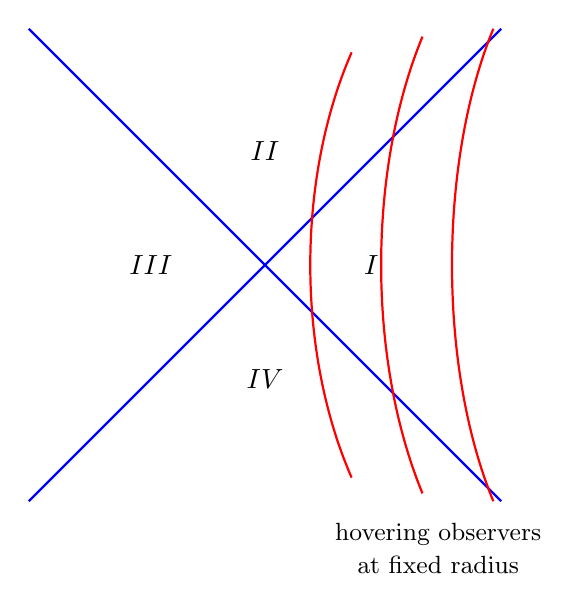
\begin{tikzpicture}[scale=1.0]
\draw[thick,blue] (-3,3) -- (3,-3);
\draw[thick,blue] (-3,-3) -- (3,3);

\draw[red,thick] (1.1,-2.7) .. controls (0.4,-1.1) and (0.4,1.1) .. (1.1,2.7);
\draw[red,thick] (2.0,-2.9) .. controls (1.3,-1.2) and (1.3,1.2) .. (2.0,2.9);
\draw[red,thick] (2.9,-3.0) .. controls (2.2,-1.3) and (2.2,1.3) .. (2.9,3.0);

\node at (1.35,0.0) {$I$};
\node at (0.0,1.45) {$II$};
\node at (-1.45,0.0) {$III$};
\node at (0.0,-1.45) {$IV$};

\node[align=center] at (2.2,-3.6) {\small hovering observers\\\small at fixed radius};
\end{tikzpicture}
\caption{Clean redraw of the Kruskal-style causal structure used in the recap. Region \(I\) is the exterior, region \(II\) the inescapable interior, and regions \(III\) and \(IV\) belong to the formal extension that will later be discarded for a real collapsing black hole.}
\end{figure}

This is already enough to say what a black hole does. In the exterior region \(I\), objects and signals may go inward, but they may also remain outside or turn back out. In region \(II\), by contrast, the causal verdict is fixed. The transcript is garbled in part of this discussion, but the secure point is clear: once one is in the interior, there is no future-directed causal path back to the exterior. To escape from region \(II\) into either outside region would require a trajectory shallower than \(45^\circ\) somewhere, and therefore faster than light. Every allowed future timelike trajectory ends on the singularity.

This opening recap is not merely repetition. It prepares the chapter's main theme. The Kruskal picture is useful, but not all of it is physically meaningful for a real black hole.

\section{Why Compactify? From Infinite Spacetime to a Finite Blackboard}

The next move is methodological. The null directions in these diagrams run off to infinity, and so does time itself. We therefore cannot draw the whole spacetime on an ordinary blackboard unless we change coordinates. The lecturer's motivation is very concrete: if we want to see everything at once and reason about the global causal structure, we need a way to compress an infinite spacetime into a finite region while keeping light rays recognizable.

He therefore backs up to the easy case, good old flat spacetime. Because the problems of interest are spherically symmetric, we suppress the angular directions and keep only time and the radial coordinate. We use coordinates \(T\) and \(R\), with
\[
R\ge 0,
\]
since negative radial distance has no meaning in polar coordinates. We also choose units in which
\[
c=1.
\]
With that convention, radial null motion is drawn at \(45^\circ\).

Before introducing the compactifying map, the lecture takes some time to orient us in the \(T\)-\(R\) plane. One draws the time axis, the radial axis, a few constant-time slices \(T=0,\pm1,\pm2\), and a few constant-radius lines \(R=1,2,3\). This is not dead formalism. It gives us landmarks, and it makes clear which features we want to preserve when the diagram is later squeezed into finite size.

There is also a subtle but important pedagogical point about the origin. In the reduced radial picture, a light ray aimed exactly at \(R=0\) appears to bounce from the origin and come back out. But nothing is physically reflecting from a wall. In the full spherically symmetric geometry the ray simply passes through the origin and emerges on the other side. The apparent bounce is only a consequence of working with the half-plane \(R\ge 0\).

Likewise, a light ray that misses the origin starts by looking almost the same, reaches a point of closest approach, and then turns back outward. In these coordinates it may even look as if something has repelled it from the origin. But that too is a coordinate description of the familiar angular-momentum barrier, not a new force. The lecturer lingers over these examples because he wants the audience to trust the diagram before he deforms it.

Now comes the essential move. We are going to squeeze and stretch the picture, but keep one thing fixed: radial light rays must remain \(45^\circ\) lines. That is the whole point of the compactification.

\section{Flat Spacetime in Null Coordinates and Penrose Form}

To make the deformation precise, we introduce null coordinates. This is the mathematically clean part of the lecture, and the board makes the move explicit.

\begin{figure}[htbp]
\centering

\includegraphics[width=0.82\textwidth]{lecture_08_figure_03.png}
\caption{Board derivation of the null-coordinate combinations \(T+R=T^+\) and \(T-R=T^-\), together with the associated \(T\)-\(R\) sketch.}
\end{figure}

We define
\begin{align}
T^+ &= T+R, \\
T^- &= T-R.
\end{align}
These are adapted to radial null motion. An ingoing radial light ray has \(T^+=\text{const}\), while an outgoing radial light ray has \(T^-=\text{const}\).

\paragraph{Worked derivation.}
The line \(R=0\) becomes particularly simple in these coordinates. Indeed,
\begin{align}
R=0
&\iff T+R=T-R \\
&\iff T^+=T^-.
\end{align}
So the entire timelike boundary \(R=0\) is described by the single relation
\begin{equation}
R=0 \iff T^+=T^-.
\end{equation}

\begin{figure}[htbp]
\centering
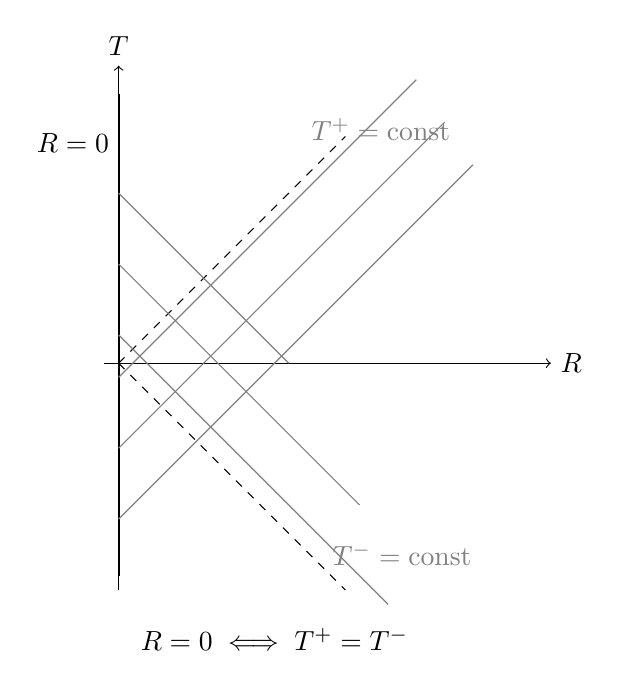
\begin{tikzpicture}[scale=0.9]
\draw[->] (-0.2,0) -- (6.1,0) node[right] {$R$};
\draw[->] (0,-3.2) -- (0,4.2) node[above] {$T$};

\draw[thick] (0,-3.0) -- (0,3.8);
\node[left] at (0,3.1) {$R=0$};

\draw[dashed] (0,0) -- (3.2,3.2);
\draw[dashed] (0,0) -- (3.2,-3.2);

\draw[gray] (0,2.4) -- (2.4,0);
\draw[gray] (0,1.4) -- (3.4,-2.0);
\draw[gray] (0,0.4) -- (3.8,-3.4);

\draw[gray] (0,-2.2) -- (5.0,2.8);
\draw[gray] (0,-1.2) -- (4.6,3.4);
\draw[gray] (0,-0.2) -- (4.2,4.0);

\node[gray] at (3.7,3.3) {$T^+=\mathrm{const}$};
\node[gray] at (4.0,-2.7) {$T^-=\mathrm{const}$};

\node at (2.2,-3.9) {$R=0 \iff T^+=T^-$};
\end{tikzpicture}
\caption{A clean \(T\)-\(R\) redraw. The two null families are the level sets of \(T^+\) and \(T^-\), and the line \(R=0\) is equivalently \(T^+=T^-\).}
\end{figure}

Now we compactify. We introduce two new null coordinates \(U^\pm\), each obtained from the corresponding \(T^\pm\) by the same bounded monotone function \(F\):
\begin{align}
U^+ &= F(T^+), &
U^- &= F(T^-),
\end{align}
with
\begin{equation}
F(+\infty)=1,
\qquad
F(-\infty)=-1.
\end{equation}
The lecture's convenient choice is
\begin{equation}
F(x)=\tanh x,
\end{equation}
so that
\begin{equation}
U^+ = \tanh(T^+),
\qquad
U^- = \tanh(T^-).
\end{equation}
There is nothing sacred about the hyperbolic tangent. It is simply a smooth function with the right limiting behavior, and so it squeezes infinite coordinate ranges down to finite ones.

The null structure is preserved for a simple reason. If an ingoing radial light ray has \(T^+=\text{const}\), then
\[
U^+=F(T^+)=\text{const},
\]
and similarly if an outgoing radial light ray has \(T^-=\text{const}\), then
\[
U^-=F(T^-)=\text{const}.
\]
Thus the compactification separately reparametrizes the two null directions, and radial light rays remain \(45^\circ\) lines. The origin line is carried along just as cleanly:
\[
T^+=T^- \Longrightarrow U^+=U^-.
\]

At this point the infinite half-plane of flat spacetime has been compressed to a finite triangle. The lecture then teaches us how to read its edges. Spatial infinity collapses to a single point \(i^0\). Future and past timelike infinities are \(i^+\) and \(i^-\). The two null edges are \(\mathscr I^+\) and \(\mathscr I^-\), often pronounced scri-plus and scri-minus, the places where incoming and outgoing light rays begin and end.

\begin{figure}[htbp]
\centering
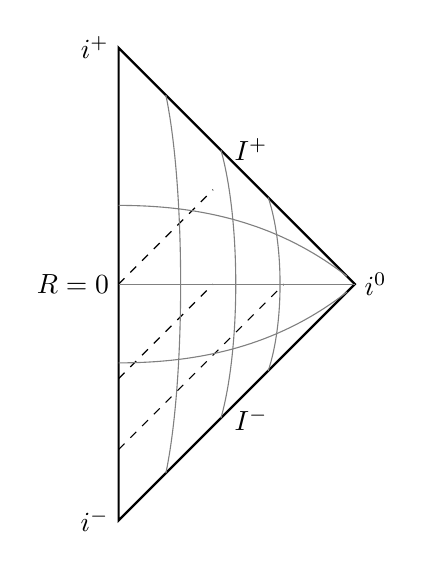
\begin{tikzpicture}[scale=1.0]
\draw[thick] (0,-3) -- (0,3) -- (3,0) -- cycle;

\node[left] at (0,3) {$i^+$};
\node[left] at (0,-3) {$i^-$};
\node[right] at (3,0) {$i^0$};
\node[left] at (0,0) {$R=0$};
\node[above right] at (1.35,1.45) {$\mathscr I^+$};
\node[below right] at (1.35,-1.45) {$\mathscr I^-$};

\draw[dashed] (0,-2.1) -- (2.1,0.0);
\draw[dashed] (0,-1.2) -- (1.2,0.0);
\draw[dashed] (0,0.0) -- (1.2,1.2);

\draw[gray] (0,0) -- (3,0);
\draw[gray] (0,1.0) .. controls (1.0,1.0) and (2.0,0.8) .. (2.9,0.1);
\draw[gray] (0,-1.0) .. controls (1.0,-1.0) and (2.0,-0.8) .. (2.9,-0.1);

\draw[gray] (0.6,-2.4) .. controls (0.85,-1.2) and (0.85,1.2) .. (0.6,2.4);
\draw[gray] (1.3,-1.7) .. controls (1.55,-0.8) and (1.55,0.8) .. (1.3,1.7);
\draw[gray] (1.9,-1.1) .. controls (2.1,-0.5) and (2.1,0.5) .. (1.9,1.1);
\end{tikzpicture}
\caption{Transcript-backed reconstruction of the Penrose diagram for radially reduced flat spacetime. Constant-time curves run outward toward \(i^0\), while constant-radius curves rise from \(i^-\) toward \(i^+\).}
\end{figure}

One last point from the lecture should be kept in mind. These diagrams do \emph{not} preserve metric size. They preserve causal structure. That is the invariant we are after.

\section{The Compactified Schwarzschild Geometry}

Armed with the flat-space construction, we now return to the black hole and do the same thing again. We compactify the Kruskal geometry by introducing null coordinates and squeezing the infinite ranges into a finite figure. The lecturer describes the result as a diagonal rectangle or diamond-like causal picture: the horizon appears as a null boundary, the exterior hovering worldlines stay outside it, and the interior region terminates on a singularity that is now visible on the page.

The crucial physical point is that the singularity is \emph{not} at infinity in the infalling observer's experience. Once the horizon is crossed, the remaining proper time before striking the singularity is finite. The Penrose diagram makes this visually unavoidable.

The horizon is again identified by the Schwarzschild condition
\begin{equation}
1-\frac{2MG}{r}=0
\qquad \Longleftrightarrow \qquad
r=2MG.
\end{equation}
This is the same distinguished radius at which the Schwarzschild factor changes sign.

\begin{figure}[htbp]
\centering

\includegraphics[width=0.72\textwidth]{lecture_08_figure_04.png}
\caption{Board sketch contrasting the formal extended picture with the physically relevant black-hole region. The red label \emph{singularity} is explicit on the board.}
\end{figure}

\begin{figure}[htbp]
\centering
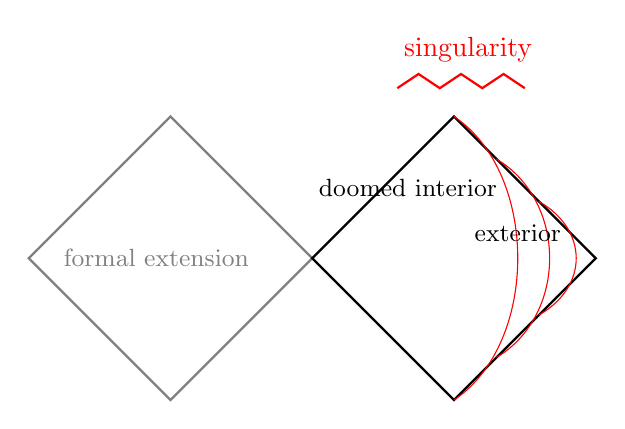
\begin{tikzpicture}[scale=0.9]
\draw[gray,thick] (-4,0) -- (-2,2) -- (0,0) -- (-2,-2) -- cycle;
\draw[thick] (0,0) -- (2,2) -- (4,0) -- (2,-2) -- cycle;

\draw[red,thick] (1.2,2.4) -- (1.5,2.6) -- (1.8,2.4) -- (2.1,2.6) -- (2.4,2.4) -- (2.7,2.6) -- (3.0,2.4);
\node[red] at (2.2,2.95) {singularity};

\draw[red] (2.0,-2.0) .. controls (3.2,-1.2) and (3.2,1.2) .. (2.0,2.0);
\draw[red] (2.6,-1.4) .. controls (3.6,-0.8) and (3.6,0.8) .. (2.6,1.4);
\draw[red] (3.2,-0.8) .. controls (3.9,-0.4) and (3.9,0.4) .. (3.2,0.8);

\node at (2.9,0.35) {\small exterior};
\node at (1.35,1.0) {\small doomed interior};
\node[gray] at (-2.2,0.0) {\small formal extension};
\end{tikzpicture}
\caption{A conservative redraw of the causal picture emphasized in the lecture: the surviving exterior, the doomed interior, the future singularity, and the contrast with the extra formal part of the extension.}
\end{figure}

The lecture is very direct here. If you are in the exterior, you may still escape, or you may fall in. If you are in the interior, you are doomed. The diagram is already saying everything important about future-directed causal motion.

\subsection{Question \& Answer}

\paragraph{Question.} What are quadrants \(III\) and \(IV\), and do they belong to a real black hole?

\paragraph{Answer.} As parts of the maximally extended Kruskal solution, they are legitimate pieces of the formal analytic extension. One may read region \(III\) as another exterior region and region \(IV\) as its time-reversed companion. The lecturer does not deny their mathematical existence. But his point is that a real black hole formed by collapse does not contain them. The physical black hole keeps the causal lesson of the exterior and the doomed interior, and discards the rest. The left-hand side of the full Kruskal diagram is mathematically instructive but physically absent in the collapse problem.

\section{Spatial Slices, Two-Spheres, and the Einstein--Rosen Bridge}

The lecture then freezes the compactified diagram on a spacelike slice and asks what that slice looks like as \emph{space} rather than spacetime. This is where the wormhole image enters, and this is also where the notes must be careful not to let the picture outrun the causal argument.

Because the angular directions have been suppressed, each point of the radial diagram actually stands for a two-sphere. At Schwarzschild radius \(r\), that sphere has area
\begin{equation}
A=4\pi r^2.
\end{equation}
So a spacelike slice through the extended Schwarzschild geometry is not a one-dimensional curve in the full geometry. It is a family of two-spheres whose size changes as one moves along the slice.

Far away the spheres are very large. As one moves inward, their radius shrinks until it reaches a minimum at the horizon,
\begin{equation}
r_{\min}=2MG.
\end{equation}
If one keeps going through the formal extension, the spheres expand again toward another asymptotic side. This is the Einstein--Rosen bridge picture.

\begin{figure}[htbp]
\centering

\includegraphics[width=0.72\textwidth]{lecture_08_figure_05.png}
\caption{Board sketch of the bridge geometry. The visible Schwarzschild factor fragment at upper left ties the picture to the distinguished radius \(r=2MG\).}
\end{figure}

The board only shows part of the relevant Schwarzschild factor,
\begin{equation}
1-\frac{2MG}{r},
\end{equation}
but the transcript makes clear what is needed: the throat occurs at the same special radius \(r=2MG\).

\begin{figure}[htbp]
\centering
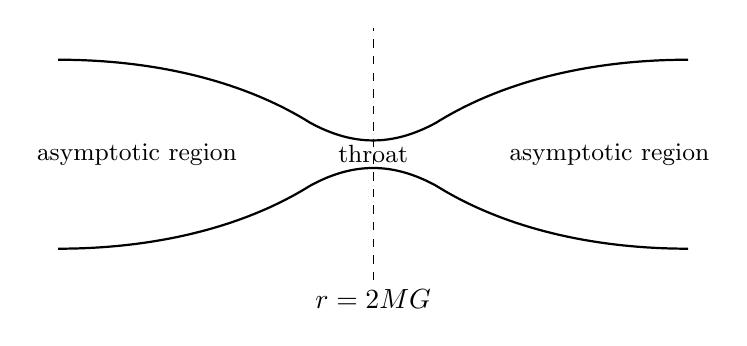
\begin{tikzpicture}[scale=1.0]
\draw[thick] (-4,1.2)
.. controls (-2.7,1.2) and (-1.6,0.9) .. (-0.8,0.4)
.. controls (-0.25,0.1) and (0.25,0.1) .. (0.8,0.4)
.. controls (1.6,0.9) and (2.7,1.2) .. (4,1.2);

\draw[thick] (-4,-1.2)
.. controls (-2.7,-1.2) and (-1.6,-0.9) .. (-0.8,-0.4)
.. controls (-0.25,-0.1) and (0.25,-0.1) .. (0.8,-0.4)
.. controls (1.6,-0.9) and (2.7,-1.2) .. (4,-1.2);

\draw[dashed] (0,-1.6) -- (0,1.6);
\node[below] at (0,-1.6) {$r=2MG$};
\node at (0,0) {\small throat};
\node at (-3.0,0) {\small asymptotic region};
\node at (3.0,0) {\small asymptotic region};
\end{tikzpicture}
\caption{Schematic spatial slice through the extended Schwarzschild geometry. This is a cautious reconstruction of the lecture's bridge picture, not a literal embedding calculation.}
\end{figure}

Now comes the correction. The slice suggests a bridge between two asymptotic regions, and so it invites the thought that one might travel from one universe to the other by passing through the neck. The lecture first lets that suggestion appear, and then kills it causally. To get from one exterior region to the other, a worldline would have to become shallower than a \(45^\circ\) null line somewhere on the Penrose diagram. That is forbidden. So the Einstein--Rosen bridge is non-traversable.

The lecturer also emphasizes why the spatial picture can mislead. It is a picture of \emph{space at an instant of time}; but there is simply not enough causal time to get through. One can say, loosely, that the bridge opens and closes before anything can cross it. Better still, one simply looks back at the Penrose diagram and reads off the causal answer.

\section{Building a Real Black Hole from an Infalling Null Shell}

At this point the lecture changes problem completely. We are no longer reading off the properties of an eternal black hole. We are constructing a real one.

The model is chosen for simplicity. We imagine not a collapsing star with messy internal structure, but a thin spherical shell of incoming radiation. It is a shell of light, and therefore moves inward at the speed of light. At sufficiently small radius the energy on that shell is concentrated tightly enough that a black hole forms.

The second ingredient is the shell theorem in its general-relativistic form.

\begin{remark}
For the spherically symmetric shell used in this lecture, the interior region is flat spacetime, while the exterior region is Schwarzschild. This is the operational shell theorem, or Birkhoff-type statement, used by the lecture. It is not proved here.
\end{remark}

The lecturer motivates this by first recalling the Newtonian shell theorem: inside a spherical shell there is no gravitational field, while outside the shell the field is the same as that of a point mass at the center. He then states the corresponding relativistic version in the only form needed here: the inside is flat, the outside is Schwarzschild. The shell may move; the rule is the same.

That is enough to construct the collapse spacetime. The shell itself is null, so it must be drawn at \(45^\circ\). On one side of that null line the geometry is flat. On the other side it is Schwarzschild. We can summarize the rule as
\begin{equation}
\text{inside shell} = \text{flat spacetime},
\qquad
\text{outside shell} = \text{Schwarzschild geometry}.
\end{equation}

The gluing prescription then becomes almost embarrassingly simple:

\begin{enumerate}
\item Draw the flat Penrose diagram and keep only the region interior to the incoming shell.
\item Draw the Schwarzschild Penrose diagram and keep only the region exterior to that same shell.
\item Throw away the wrong pieces.
\item Sew the two surviving pieces together along the shell trajectory.
\end{enumerate}

This is exactly how the lecture proceeds on the board: discard the wrong half of one picture, discard the wrong half of the other, and glue the right halves along the shell.

\begin{figure}[htbp]
\centering
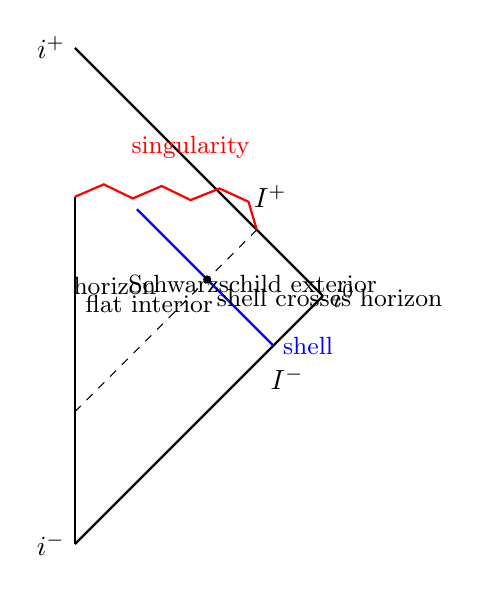
\begin{tikzpicture}[scale=1.05]
\coordinate (im) at (0,-3.0);
\coordinate (ip) at (0,3.0);
\coordinate (i0) at (3.0,0.0);
\coordinate (S)  at (0,1.2);
\coordinate (E)  at (2.2,0.8);
\coordinate (P)  at (2.4,-0.6);
\coordinate (Q)  at (0.75,1.05);
\coordinate (H)  at (0,-1.4);
\coordinate (X)  at (1.6,0.2);

\draw[thick] (im) -- (S);
\draw[thick] (im) -- (i0);
\draw[thick] (ip) -- (i0);

\draw[red,thick] (S) -- (0.35,1.35) -- (0.7,1.18) -- (1.05,1.33) -- (1.4,1.16) -- (1.75,1.30) -- (2.1,1.14) -- (E);
\node[red,above] at (1.4,1.55) {\small singularity};

\draw[thick,blue] (P) -- (Q);
\node[blue,right] at (P) {\small shell};

\draw[dashed] (H) -- (E);
\node[above left] at (1.1,-0.1) {\small horizon};

\filldraw (X) circle (1.2pt);
\node[below right] at (X) {\small shell crosses horizon};

\node at (0.9,-0.1) {\small flat interior};
\node at (2.15,0.15) {\small Schwarzschild exterior};

\node[left] at (im) {$i^-$};
\node[left] at (ip) {$i^+$};
\node[right] at (i0) {$i^0$};
\node[below right] at (2.25,-0.75) {$\mathscr I^-$};
\node[above right] at (2.05,0.95) {$\mathscr I^+$};
\end{tikzpicture}
\caption{Transcript-backed reconstruction of the collapse geometry. The shell is an ingoing null line; flat spacetime is kept on its interior side and Schwarzschild geometry on its exterior side.}
\end{figure}

The shell itself experiences nothing special at the moment when it is merely crossing from the flat part of the diagram into the Schwarzschild part. It is a lightlike shell, and it continues inward until it reaches the singularity. The essential structure is not carried by local drama on the shell; it is carried by the causal organization of the glued spacetime.

\section{Horizon Before Arrival: The Event-Horizon Puzzle}

Now comes the conceptual climax of the lecture. Once the collapse spacetime has been built, the natural question is: where is the horizon? Or, as the lecturer puts it, where is the point of no return?

\begin{definition}
The event horizon is the boundary between those events that can still send a future-directed causal signal to \(\mathscr I^+\) and those that cannot.
\end{definition}

The lecture finds it diagrammatically. Start at the corner where the singularity meets future null infinity, and trace a \(45^\circ\) null line backward. That backward-traced null line is the event horizon.

But the lecturer then insists on a second point, and it is the one that makes students uneasy. The horizon does not simply appear at the moment when the shell crosses its own Schwarzschild radius and then stay put. In the enlarged board drawing, the horizon begins as a tiny trapped region near the center, expands outward through a part of spacetime that is still flat, and only later meets the incoming shell. At that meeting event the shell passes its own Schwarzschild radius. Above that event, the horizon is the ordinary constant-radius horizon of the completed black hole.

\begin{figure}[htbp]
\centering
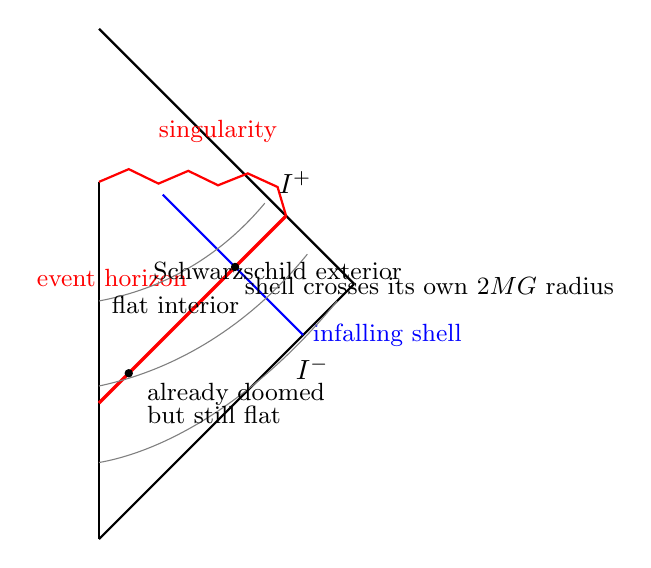
\begin{tikzpicture}[scale=1.08]
\coordinate (im) at (0,-3.0);
\coordinate (ip) at (0,3.0);
\coordinate (i0) at (3.0,0.0);
\coordinate (S)  at (0,1.2);
\coordinate (E)  at (2.2,0.8);
\coordinate (P)  at (2.4,-0.6);
\coordinate (Q)  at (0.75,1.05);
\coordinate (H)  at (0,-1.4);
\coordinate (X)  at (1.6,0.2);
\coordinate (D)  at (0.35,-1.05);

\draw[thick] (im) -- (S);
\draw[thick] (im) -- (i0);
\draw[thick] (ip) -- (i0);

\draw[red,thick] (S) -- (0.35,1.35) -- (0.7,1.18) -- (1.05,1.33) -- (1.4,1.16) -- (1.75,1.30) -- (2.1,1.14) -- (E);
\node[red,above] at (1.4,1.55) {\small singularity};

\draw[very thick,red] (H) -- (E);
\node[red,above left] at (1.15,-0.15) {\small event horizon};

\draw[thick,blue] (P) -- (Q);
\node[blue,right] at (P) {\small infalling shell};

\filldraw (X) circle (1.2pt);
\node[below right] at (X) {\small shell crosses its own \(2MG\) radius};

\draw[gray] (0.0,-2.1) .. controls (0.85,-1.95) and (1.9,-1.3) .. (2.8,-0.2);
\draw[gray] (0.0,-1.2) .. controls (0.95,-1.0) and (1.8,-0.45) .. (2.45,0.35);
\draw[gray] (0.0,-0.2) .. controls (0.8,-0.05) and (1.45,0.35) .. (1.95,0.95);

\filldraw (D) circle (1.2pt);
\node[below right] at (0.45,-1.05) {\small already doomed};
\node[below right] at (0.45,-1.32) {\small but still flat};

\node at (0.9,-0.25) {\small flat interior};
\node at (2.1,0.15) {\small Schwarzschild exterior};

\node[below right] at (2.2,-0.75) {$\mathscr I^-$};
\node[above right] at (2.0,0.95) {$\mathscr I^+$};
\end{tikzpicture}
\caption{A second transcript-backed reconstruction of the collapse diagram, now emphasizing the backward-traced event horizon. Part of the horizon lies in a region that is still locally flat and has not yet been reached by the shell.}
\end{figure}

This is the striking effect on which the lecture dwells. Part of the horizon lies in flat spacetime. The shell has not yet arrived there. An observer there may feel nothing unusual, may see no incoming shell on the backward light cone, and yet may already be doomed. The reason is not local and it is not mechanical. It is global and causal.

\subsection{Question \& Answer}

\paragraph{Question.} How can an observer already be doomed in flat spacetime, before the shell has reached them?

\paragraph{Answer.} Because the horizon is not a material membrane. It is the global boundary between escape and no escape. Inside the shell the geometry may still be flat, and crossing the shell may be the first locally noticeable encounter with matter or radiation. But the event horizon is defined by the entire future of the spacetime. If from a given event no future-directed causal curve reaches \(\mathscr I^+\), then that event lies inside the horizon even if locally nothing dramatic has happened yet.

The lecture then presses the issue harder. ``Before'' according to which time? The answer is that time is just a coordinate. An instant of time means a chosen spacelike slice. One may foliate the spacetime in different ways, and the shell may be outside the horizon on one slice and inside it on another. The causal conclusion does not change. Different slicings change simultaneity, not the escape structure.

This is why the lecturer insists that crossing the shell and crossing the horizon are different things. Crossing the shell can involve actual matter or radiation, and therefore can in principle be locally noticeable. Crossing the horizon need not involve any local drama at all. The horizon is, in that sense, ghostly: it has causal significance without being a material surface.

There is also an important practical corollary. Being inside the shell is not by itself fatal. One may be inside the shell and still outside the horizon, in which case the shell can pass by and one may yet escape. The students press exactly this point late in the lecture, and the answer is yes: if you are far enough from the eventual center and still outside the horizon, you can simply let the shell cross you. It may do damage as matter or radiation, but that is a separate issue. The real issue is whether you are inside the causal no-return boundary.

The mirror thought experiments sharpen the same distinction. A reflecting structure built sufficiently early and sufficiently far out can change the causal story. But once an observer is too deep inside the backward-traced horizon, there is no longer enough causal time to put the mirror where it must be. A mirror placed inside the horizon is merely another doomed object. The light, the mirror, and the observer all wind up at the singularity.

Finally, the proper-time statement must be kept straight. From a generic horizon-crossing event to the singularity there is only a finite proper time. Only the ideal corner where the singularity meets \(\mathscr I^+\) is infinitely far away, and trying to cling to that corner would require infinite acceleration and infinite energy. It is not an escape route.

The lecture ends almost polemically here. If we try to reason this out without the picture, we get confused. If we draw the diagram, the answer is plain.

\section{Summary}

The chapter has followed the lecture's arc closely. We began with the near-horizon Kruskal picture: local flatness, \(45^\circ\) null directions, hovering observers in the exterior, and the inescapability of the interior. We then stepped back to flat spacetime and learned how to compactify it: first by introducing null coordinates \(T^\pm\), then by replacing them with bounded null coordinates \(U^\pm\). That gave us a finite Penrose diagram without sacrificing the causal role of light rays.

Once that machinery was in hand, we returned to the Schwarzschild geometry. The compactified black-hole diagram made the singularity finite in infalling proper time, identified the horizon again at \(r=2MG\), and exposed the extra Kruskal quadrants as formal features that do not survive in the real collapse problem. The spacelike slice through the extended geometry then produced the Einstein--Rosen bridge picture, which had to be immediately corrected by the causal argument that it is non-traversable.

Only after all that did we build a real black hole. The collapsing null shell let us glue flat interior geometry to Schwarzschild exterior geometry. From that glued spacetime we located the event horizon by tracing a null line backward from the corner where the singularity meets \(\mathscr I^+\). The resulting puzzle was the deep one: the horizon extends into a region that is still flat and has not yet been reached by the shell. The lecture's answer is the final moral of the chapter. Penrose diagrams do not faithfully represent size. They faithfully represent causal structure. And for black holes, that is the structure we must understand.